\documentclass[a4paper,twoside]{memoir}
% Set up encoding
\usepackage[utf8]{inputenc}

% Mulighed for at definere acronyms
\usepackage{acronym}

% Load up bibliography.
\usepackage[authoryear]{natbib}
\setcitestyle{numbers,square}
% Bibliography style.
\bibliographystyle{plainnat}

% Algorithm support.
\usepackage{algorithmic}
\usepackage{algorithm}
\usepackage{subfig}
\usepackage{amsmath}
\usepackage{amsfonts}
% Make algorithms appear as procedures instead.
\floatname{algorithm}{Procedure}
\renewcommand{\algorithmicrequire}{\textbf{Input:}}
\renewcommand{\algorithmicensure}{\textbf{Output:}}

% Image frames.
\setlength{\fboxsep}{0pt}
\setlength{\fboxrule}{0.5pt}

% Also, images.
\usepackage{graphicx}

% tabeller der strækker sig over flere sider
\usepackage{longtable}

% flere tabel-muligheder
\usepackage{multirow}

% bedre enumerate
\usepackage{enumitem}

% Todo notes here and there.
% write instead for disable: \usepackage[disable]{todonotes}
\usepackage{todonotes}

% Forbedrede floats.
\usepackage{float}
\usepackage{rotating}

% Special symbols availability.
\usepackage{amssymb}

%Degree symbol
\usepackage{gensymb}

% Wrap figure
\usepackage{wrapfig}

%landscape mode
\usepackage{lscape}

%Fun with captions
\usepackage{caption}

% Operationel semantik
\newcommand{\lag}{\langle}
\newcommand{\rag}{\rangle}
\newcommand{\setof}[2]{\ensuremath{\{ #1 \mid #2 \}}}
\newcommand{\set}[1]{\ensuremath{\{ #1 \}}}
\newcommand{\besk}[1]{\ensuremath{\lag #1 \rag}}
\newcommand{\ra}{\rightarrow}
\newcommand{\lra}{\longrightarrow}
\newcommand{\Ra}{\Rightarrow}

% CODE %
\usepackage{listings}
\usepackage{color}
%\usepackage{bera}
\definecolor{gray}{rgb}{0.4,0.4,0.4}
\definecolor{darkblue}{rgb}{0.0,0.0,0.6}
\definecolor{cyan}{rgb}{0.0,0.6,0.6}
\lstset{
  basicstyle=\ttfamily,
  columns=fullflexible,
  showstringspaces=false,
  commentstyle=\color{gray}\upshape,
  basicstyle=\small,
  numberstyle=\footnotesize,
  numbers=left,
  captionpos=b,
  stepnumber=1,
  numbersep=10pt,
  tabsize=2,
  breaklines=true,
}
% Define markup of XML
\lstdefinelanguage{XML}
{
  morestring=[b]",
  morestring=[s]{>}{<},
  morecomment=[s]{<?}{?>},
  identifierstyle=\color{darkblue},
  keywordstyle=\color{cyan},
  morekeywords={id, target, type, category, value, point, correct, rows, width, time}% list your attributes here
}
% Define markup of C#
\lstdefinelanguage{CSharp}[Visual]{C++}
{
	identifierstyle=\color{darkblue},
	commentstyle=\color{green!70!black}\itshape ,
	stringstyle=\color{gray},
	sensitive=true,
	morestring=[b]",
	morestring=[b]',
	morecomment=[l]//,
	morecomment=[n]{/*}{*/}
}

% Define markup of Javascript
\lstdefinelanguage{JavaScript}{
  keywords={typeof, new, true, false, catch, function, return, null, catch, switch, var, if, in, while, do, else, case, break},
  keywordstyle=\color{blue}\bfseries,
  ndkeywords={class, export, boolean, throw, implements, import, this},
  ndkeywordstyle=\color{darkgray}\bfseries,
  identifierstyle=\color{black},
  sensitive=false,
  comment=[l]{//},
  morecomment=[s]{/*}{*/},
  commentstyle=\color{purple}\ttfamily,
  stringstyle=\color{red}\ttfamily,
  morestring=[b]',
  morestring=[b]"
}

% Define markup of JSON
\colorlet{punct}{red!60!black}
\definecolor{background}{HTML}{EEEEEE}
\definecolor{delim}{RGB}{20,105,176}
\colorlet{numb}{magenta!60!black}
\lstdefinelanguage{json}{
    basicstyle=\normalfont\ttfamily,
    numbers=left,
    numberstyle=\scriptsize,
    stepnumber=1,
    numbersep=8pt,
    showstringspaces=false,
    breaklines=true,
    frame=lines,
    backgroundcolor=\color{background},
    literate=
     *{0}{{{\color{numb}0}}}{1}
      {1}{{{\color{numb}1}}}{1}
      {2}{{{\color{numb}2}}}{1}
      {3}{{{\color{numb}3}}}{1}
      {4}{{{\color{numb}4}}}{1}
      {5}{{{\color{numb}5}}}{1}
      {6}{{{\color{numb}6}}}{1}
      {7}{{{\color{numb}7}}}{1}
      {8}{{{\color{numb}8}}}{1}
      {9}{{{\color{numb}9}}}{1}
      {:}{{{\color{punct}{:}}}}{1}
      {,}{{{\color{punct}{,}}}}{1}
      {\{}{{{\color{delim}{\{}}}}{1}
      {\}}{{{\color{delim}{\}}}}}{1}
      {[}{{{\color{delim}{[}}}}{1}
      {]}{{{\color{delim}{]}}}}{1},
}

\lstdefinelanguage{KAPAOOW}{
 sensitive=false,
 keywords={character, characters, action, end, if, then, else, from, to, downto, next, while, loop, use, turn, begins, ends, select, wins, draw, random, of, case, cases, enemy, player, start, skip, attack, types, damage, defend, by, using, message, and, or, is, value, mod},
 identifierstyle=\itshape,
 keywordstyle=\bfseries,
 stringstyle=\normalfont,
 morestring=[b]",
 comment=[l]{//},
 commentstyle=\color{gray}
}

% Neat-o referencer...o.
\usepackage{bookmark,hyperref}
\usepackage{nameref}

% hack fra nettet.
% http://tex.stackexchange.com/questions/1230/reference-name-of-description-list-item-in-latex
\makeatletter
\let\orgdescriptionlabel\descriptionlabel
\renewcommand*{\descriptionlabel}[1]{
  \let\orglabel\label
  \let\label\@gobble
  \phantomsection
  \edef\@currentlabel{#1}
  %\edef\@currentlabelname{#1}
%  \let\label\orglabel
  \orgdescriptionlabel{#1}
}
\makeatother
% Rettehak. Meget lettere end \checkmark
\newcommand{\yes}{\checkmark}


% Create a new command, HRule, to insert some nice horisontal rules on the title page.
\newcommand{\HRule}{\rule{\linewidth}{0.3mm}}

% New command for two figures, side by side.
\newcommand{\twofigs}[6]
{
	\begin{figure}[H]
		\begin{minipage}[b]{0.5\columnwidth}
		\centering
		\includegraphics[width=0.8\columnwidth]{img/#1}
		\caption{#2\label{#3}}
		\end{minipage}
		\hspace{0.5cm}
		\begin{minipage}[b]{0.5\columnwidth}
		\centering
		\includegraphics[width=0.8\columnwidth]{img/#4}
		\caption{#5\label{#6}}
		\end{minipage}
	\end{figure}
}

% Sørg for at paragrafplads ikke spildes.
\raggedbottom

% Package til at regne forskellen ud mellem 2 labels
\usepackage{refcount}
\newcommand{\pagedifference}[2]{\number\numexpr\getpagerefnumber{#2}+1-\getpagerefnumber{#1}\relax}

\usepackage{color,calc,graphicx,soul,fourier}
\definecolor{aaublue}{RGB}{33,26,82}
\makeatletter
\newlength\dlf@normtxtw
\setlength\dlf@normtxtw{\textwidth}
\def\myhelvetfont{\def\sfdefault{mdput}}
\newsavebox{\feline@chapter}
\newcommand\feline@chapter@marker[1][4cm]{%
  \sbox\feline@chapter{%
    \resizebox{!}{#1}{\fboxsep=1pt%
      \colorbox{aaublue}{\color{white}\bfseries\sffamily\thechapter}%
    }}%
  \rotatebox{90}{%
    \resizebox{%
      \heightof{\usebox{\feline@chapter}}+\depthof{\usebox{\feline@chapter}}}%
    {!}{\scshape\so\@chapapp}}\quad%
  \raisebox{\depthof{\usebox{\feline@chapter}}}{\usebox{\feline@chapter}}%
}
\newcommand\feline@chm[1][4cm]{%
  \sbox\feline@chapter{\feline@chapter@marker[#1]}%
  \makebox[0pt][l]{% aka \rlap
    \makebox[1cm][r]{\usebox\feline@chapter}%
  }}
\makechapterstyle{daleif1}{
  \renewcommand\chapnamefont{\normalfont\Large\scshape\raggedleft\so}
  \renewcommand\chaptitlefont{\normalfont\huge\bfseries\scshape\color{aaublue}}
  \renewcommand\chapternamenum{}
  \renewcommand\printchaptername{}
  \renewcommand\printchapternum{\null\hfill\feline@chm[2.5cm]\par}
  \renewcommand\afterchapternum{\par\vskip\midchapskip}
  \renewcommand\printchaptertitle[1]{\chaptitlefont\raggedleft ##1\par}
}
\makeatother
\chapterstyle{daleif1}
\setlength\afterchapskip {\onelineskip }
\setlength\beforechapskip {\onelineskip }
\usepackage{lipsum}



\begin{document}

\begin{titlingpage}
\begin{center}
% Upper part of the page. The '~' is needed because \\
% only works if a paragraph has started.

\includegraphics[width=0.30\textwidth]{img/titelblad/AAU_logo_2012}~\\[0.5cm]

\textsc{\LARGE Aalborg University}\\[0.3cm]

\textsc{\Large Bachelor project}\\[0.5cm]

% Title
\HRule \\[0.4cm]
{ \huge \bfseries Train}\\[0.3cm]
{ \bfseries Optional subtitle}

\HRule \\[0.4cm]

% Author and supervisor
\begin{minipage}{\textwidth}
\begin{center}
	Aalborg University, Department of Computer Science\\
	P6, Spring semester 2013\\
	Project group sw606f13 / 5.1.38\\
\end{center}
\end{minipage}\\[1cm]

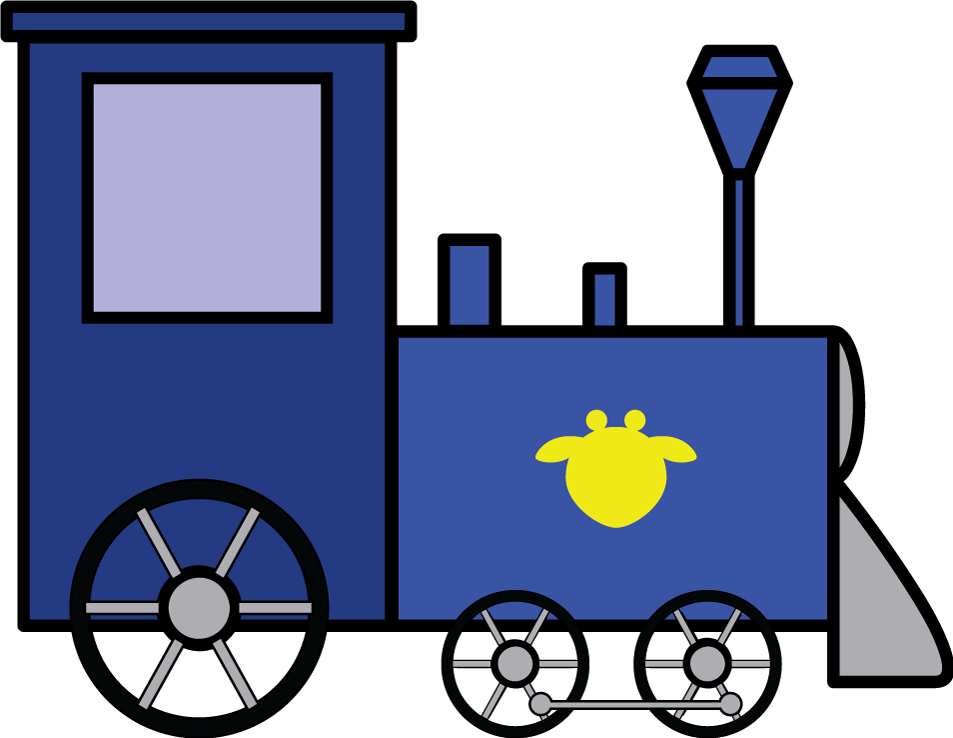
\includegraphics[width=\textwidth]{img/train}

\vfill



% Bottom of the page
{\large \today}

\end{center}
\end{titlingpage}


\newpage
\thispagestyle{empty}
\mbox{}

\thispagestyle{empty}
\begin{titlepage}
\begin{nopagebreak}
\setcounter{page}{3}
{\samepage 
\begin{tabular}{r}
\parbox{\textwidth}{  \raisebox{11mm}{
\includegraphics[height=1.2cm]{img/Titelblad/logo.jpg}}
\hfill \parbox{4.9cm}{\begin{tabular}{l}
{\sf\small \textbf{Department of Computer Science }}\\
{\sf\small  \textbf{Software Engineering}} \\
{\sf\small Selma Lagerløfs Vej 300} \\
{\sf\small Telephone +45 9940 9940} \\
{\sf\small +45 9940 9798} \\
{\sf\small http://www.cs.aau.dk}
\end{tabular}}}
\\
\end{tabular}

\begin{tabular}{cc}
\parbox{6cm}{
\begin{description}

\item {\bf Title:} 

Train
  
\item {\bf Subject:} 
Developing Complex Software Systems.

\end{description}

\parbox{8cm}{

\begin{description}
\item {\bf Project period:}\\
   P6, Spring semester 2013\\
  \hspace{4cm}
\item {\bf Project group:}\\
  SW606f13\\
  \hspace{4cm}
\item {\bf Attendees:}\\
Jacob Karstensen Wortmann \\
Jesper Riemer Andersen \\
Nicklas Andersen \\
Simon Reedtz Olesen \\

  \hspace{2cm}
\item {\bf Supervisor:}\\
Ulrik Mathias Nyman \\
\end{description}
}
\begin{description}
\item {\bf Finished:}
\item {\bf Number of pages:} \pageref{lastpage}
\item {\bf Appendix pages:} \pagedifference{appendixStart}{appendixEnd}
\end{description}
\vfill } &
\parbox{7cm}{
  \vspace{.15cm}
  \hfill 
  \begin{tabular}{l}
  {\bf Synopsis:}\bigskip \\
  \fbox{
    \parbox{6.5cm}{\bigskip
     {\vfill{\small %blank
     \bigskip}}
     }}
   \end{tabular}}
\end{tabular}}
\\ \\
\noindent{\footnotesize\emph{The content of this rapport can be used freely; however publication (with source material) may only occur in agreement with
the authors.}}
\end{nopagebreak}
\end{titlepage}
% Titelblad

\newpage
\thispagestyle{empty}
\mbox{}

\setcounter{page}{7}
\thispagestyle{empty}

\noindent\rule{8cm}{0.03cm}\\
Jacob Karstensen Wortmann\\\\

\noindent\rule{8cm}{0.03cm}\\ 
Jesper Riemer Andersen\\ \\

\noindent\rule{8cm}{0.03cm}\\
Nicklas Andersen\\\\

\noindent\rule{8cm}{0.03cm}\\
Simon Reedtz Olesen\\\\


\newpage
\thispagestyle{empty}
\mbox{}

This project was written as the Bachelor project by group SW606F13 - Software students from the Department of Computer Science at Aalborg University in the spring of 2013. The report documents the GIRAF project of 2013 and the implementation of the Train application. The application is developed for the Android platform. The reader is expected to be familiar with Java and UML. We have included our knowledge from all our previous semesters.
\\\\
When reading the report, there are a few things the reader should be aware of:
\begin{itemize}
\item When a reference to a source of a section or paragraph is given, the number of the source is written inside square brackets $[\;]$. The number is a reference to the bibliography list on page \pageref{chap:bib}.
\item When "we/us/our" is mentioned in the report, it is a referral to the authors of the report
\end{itemize}
We would like to thank our supervisor Ulrik Mathias Nyman for the feedback he has given throughout the project.


\newpage
\thispagestyle{empty}
\mbox{}

\setcounter{secnumdepth}{3}
\setcounter{tocdepth}{1}

\tableofcontents

\chapter{Introduction}\label{chap:intro}



\bookmarksetup{startatroot}% dette skulle stoppe part, så conclusion får indryk. Problemet i skrivende øjeblik er at chapters har samme indryk uafhængigt af parts
\addtocontents{toc}{\bigskip}%laver ekstra mellemrum

\section{Autism}

Autism is a spectrum disorder, which appears in the first three years of a child's life. It affects the development of the brain that has to do with social and communication skills. There are different diagnosis of autism:

\begin{description}
\item[ADHD] Attention Delficit/Hyperactivity Disorder
\item[Tourette] Verbal and motor tics
\item[Chromosomal defects]
\end{description}

Autism is a physical condition and it is linked to an abnormal chemistry in the brain, however the exact causes of these abnormalities are still unknown. 

\subsection*{Symptoms} 

Children with autism usually have a hard time with "pretend to play", they have a hard time imitating the actions of others when playing and prefer to play alone. They also have difficulties with social interaction and communication - verbally and non-verbally. 

In general people with autism may:

\begin{description}
\item Be very sensitive to sight, hearing, touch, or taste.
\item Have a very hard time adjusting to new routines and when routines are changed.
\item Show unusual attachments to objects
\end{description} 

The difficulties with social interaction means that people with autism may have a hard time starting and maintaining a social conversation, they communicate with gestures instead of words, develops language slowly and some develops none at all. 

The lack of social interaction means they might have a hard time making friends, they may be withdrawn and avoid eye contact. 

\subsection*{Signs and tests}

Some of the signs that parents might need to further test their child for autism are if the child fails to meet any of the following language milestones:

\begin{description}
\item Babbling by 12 months
\item Gesturing (such as pointing or waving goodbye) by 12 months
\item Saying single words by 16 months
\item Losing any language or social skills at any age
\end{description}

Children failing to meet any of those language milestones might receive a hearing evaluation, a blood test and a screening test for autism. Since autism includes a broad spectrum of symptoms, a single brief evaluation cannot predict what abilities the child might have, therefore a range of different skills are evaluatied, such as:

\begin{description}
\item Communication
\item Language
\item Motor skills
\item Speech
\item Success at school
\item Thinking abilities
\end{description}

Some parents might be scared of getting their child diagnosed because they are scared of labelling it, however without a diagnosis the child might not get the necessary treatment. 

\subsection*{Treatment}

Autism cannot be cured, however an early diagnosis and treatment can greatly improve the child's life. The different programs usually build on the child's interests and is highly structured as they need their routines. 

Our application was developed as a part of the GIRAF project 2013, a multi-project consisting of eight project groups, each with their own sub-project. Our focus in this project was to develop a game for GIRAF. 

The problem definition in \chapref{chap:intro} states:

\begin{quote}
\textit{"In what ways can we aid the pedagogues in their work with children with autism, by digitalizing a physical exercise onto an Android tablet?"} 
\end{quote}
The exercise we chose was an exercise that our contact person, Tove Søby, had presented during the first week of the project. The child had to place pictograms onto a train and unload them at the correct stations, this already allowed for great customization but required a lot of work from Tove Søby, so it was an ideal exercise for us to try and implement this on the Android platform. 

The main focus with our application was to make it customizable for the guardian, so that they easily can create new and different games for each child. 

We achieved this by creating a menu using LinearLayouts so they are possible to edit on runtime. The guardian is able to choose a specific child from the list and start creating a new game for that child. Using \ac{cat} they are able to choose the pictogram they want as category for each station and what pictograms they want associated with each station. This allows for customization with very limited effort from their side, which is what we wanted to achieve. 

The different graphical elements in the graphical side of the application is drawn in vector graphics, this makes it possible to resize the graphics in the future without a loss of quality. 

We have also implemented a whistle sound when the train starts driving and different random elements that can occur throughout the game, such as cows and trees on the hills in the background. This was done to create an element of surprise, which is something Tove Søby mentioned the children really liked.

Throughout the project we have communicated with Tove Søby for feedback and ideas and we have shown her and had her try out the application, however we do not have any official usability tests to document that our application is satisfactory, but we have managed to develop an application to aid the pedagogues in their work with autistic children, which was our goal for this project. 
\label{chap:conclusion}

\begin{appendices}
\label{appendixStart}

\label{appendixEnd}
\end{appendices}


% Change headings for bibliography/lists/listings. 
% Page design from fancyhdr package.
\fancyhead{}
\fancyfoot{}
\fancyhead[RO,LE]{\leftmark}
\fancyfoot[C]{\thepage}
\setlength{\headheight}{23pt}

\listoffigures
\listoftables
\lstlistoflistings

% Afslut med bibliografien. Bibliografien har mærkelige sidetal og side reference. Fixed med cleardoublepage og phantomsection
\cleardoublepage
\phantomsection
\addcontentsline{toc}{chapter}{Bibliography}
\label{chap:bib}% brugt i preface
\bibliography{bib/bibliografi}

\label{lastpage}% brugt i titelblad til total sidetal

\end{document}
